\section{Results: how does vulnerability change by 2041--2060?}\label{sec:future}

\begin{figure}[H]
\centering
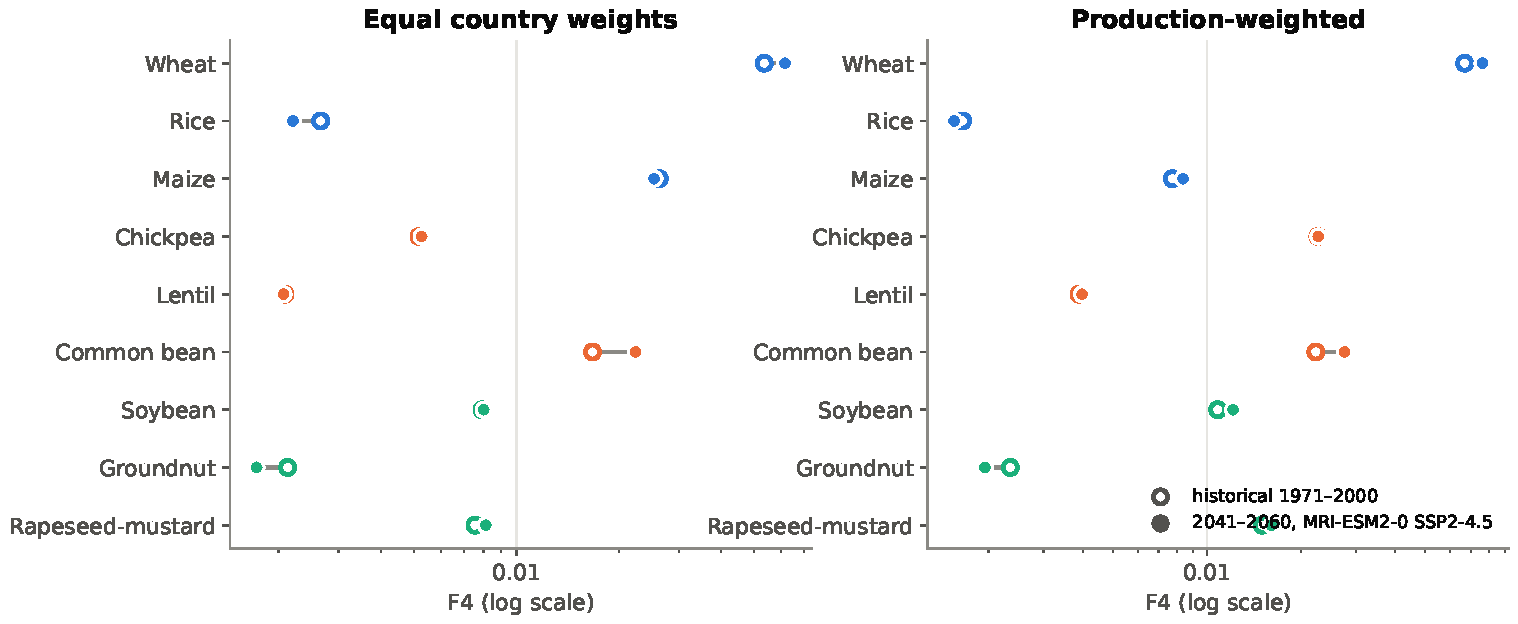
\includegraphics[width=\linewidth]{G04_present_future_crops.pdf}
\caption{Historical (1971--2000, open) and future (2041--2060, filled) crop scores, MRI-ESM2-0 SSP2-4.5, change
factors on the same years, one fixed normalisation reference.}\label{fig:future}
\end{figure}

\subsection{Magnitude and order}
Under one model and one scenario, the flowering-window effective temperature rises by \meanDTeff\,\si{\celsius} on
average over the \nPairs\ pairs.
\begin{itemize}
\item The score rises in \nPairsUp\ of \nPairs\ pairs.
\item \nPairsExceedRef\ pair exceeds the present-day reference maximum (values above one are allowed by
construction).
\item The crop order changes little: \futOrderEq\ with equal weights in 2041--2060, against \histOrderEq\ in
1971--2000 (Figure~\ref{fig:future}, Table~\ref{tab:futurecrop}).
\item Relative to 1971--2000, the equal-weighted group scores change by \grpCerealPct\% (cereals),
\grpPulsePct\% (pulses) and \grpOilseedPct\% (oilseeds). The \grpFastest\ rise fastest, mainly through common bean.
\end{itemize}

\begin{table}[H]\centering\small\caption{Crop scores 2001--24, 1971--2000 and 2041--2060 (fixed normalisation
reference; $\Delta$F4 is a change in index units, not a yield change).}\label{tab:futurecrop}
\adjustbox{max width=\linewidth}{\begin{tabular}{lrrrrrrcrrc}
\toprule
Crop & $\Delta T_{eff}$ & 2001--24 & 1971--2000 & 2041--60 & $\Delta$F4 & \% & rank eq & pairs up & F4 pw 2041--60 & rank pw \\
\midrule
Wheat & +2.0 & 0.0563 & 0.0535 & 0.0616 & +0.0080 & +15\% & 1$\to$1 & 6/6 & 0.0762 & 1$\to$1 \\
Maize & +2.0 & 0.0297 & 0.0263 & 0.0254 & -0.0009 & -3\% & 2$\to$2 & 3/6 & 0.0084 & 6$\to$6 \\
Common bean & +2.0 & 0.0172 & 0.0167 & 0.0224 & +0.0057 & +34\% & 3$\to$3 & 7/7 & 0.0276 & 3$\to$2 \\
Rapeseed-mustard & +2.0 & 0.0078 & 0.0076 & 0.0081 & +0.0006 & +8\% & 5$\to$4 & 7/7 & 0.0161 & 4$\to$4 \\
Soybean & +1.9 & 0.0078 & 0.0079 & 0.0080 & +0.0001 & +1\% & 4$\to$5 & 3/7 & 0.0121 & 5$\to$5 \\
Chickpea & +2.0 & 0.0053 & 0.0052 & 0.0053 & +0.0001 & +2\% & 6$\to$6 & 3/7 & 0.0227 & 2$\to$3 \\
Rice & +1.8 & 0.0024 & 0.0027 & 0.0022 & -0.0005 & -17\% & 7$\to$7 & 5/7 & 0.0016 & 9$\to$9 \\
Lentil & +2.2 & 0.0021 & 0.0021 & 0.0021 & -0.0000 & -1\% & 9$\to$8 & 4/7 & 0.0040 & 7$\to$7 \\
Groundnut & +1.6 & 0.0015 & 0.0021 & 0.0017 & -0.0004 & -19\% & 8$\to$9 & 2/5 & 0.0019 & 8$\to$8 \\
\bottomrule
\end{tabular}
\par\vspace{2pt}{\footnotesize MRI-ESM2-0, SSP2-4.5, change factors on 1971--2000 years; one fixed normalisation reference (2001--24 nine-crop maxima); sensitivity, importance, crop area, irrigation and calendars held fixed. $\Delta T_{eff}$ = mean change in flowering-window effective temperature (\si{\celsius}). \% only where the historical score is $\geq$1\% of the largest.}
}\end{table}

\subsection{Heat and water parts of the change}
The change splits exactly into heat and water parts (Eq.~\ref{eq:decomp}).
\begin{itemize}
\item Summed over all pairs, the heat term contributes about \futHeatShare\% of the increase and the water term
\futWaterShare\%. The future increase is mainly heat, while today's scores are mainly water.
\item The largest increase is \futTopPair\ (\futTopPairChange), about two-thirds of it through water. Wheat in
India and common bean in India, Brazil and Myanmar rise almost entirely through heat. Wheat in the USA and bean in
Tanzania rise through heat and water in similar measure (Figure~\ref{fig:futurepairs},
Table~\ref{tab:futurepairs}; pair values in \file{future\_components.csv}).
\item Every pair whose score falls does so through the water term alone. In those pairs the change factors give a
smaller rainfed deficit, while the heat term stays near zero. Examples are rice, maize, soybean and groundnut in
some countries, such as maize in South Africa and rice in Nigeria.
\end{itemize}

\begin{figure}[H]\centering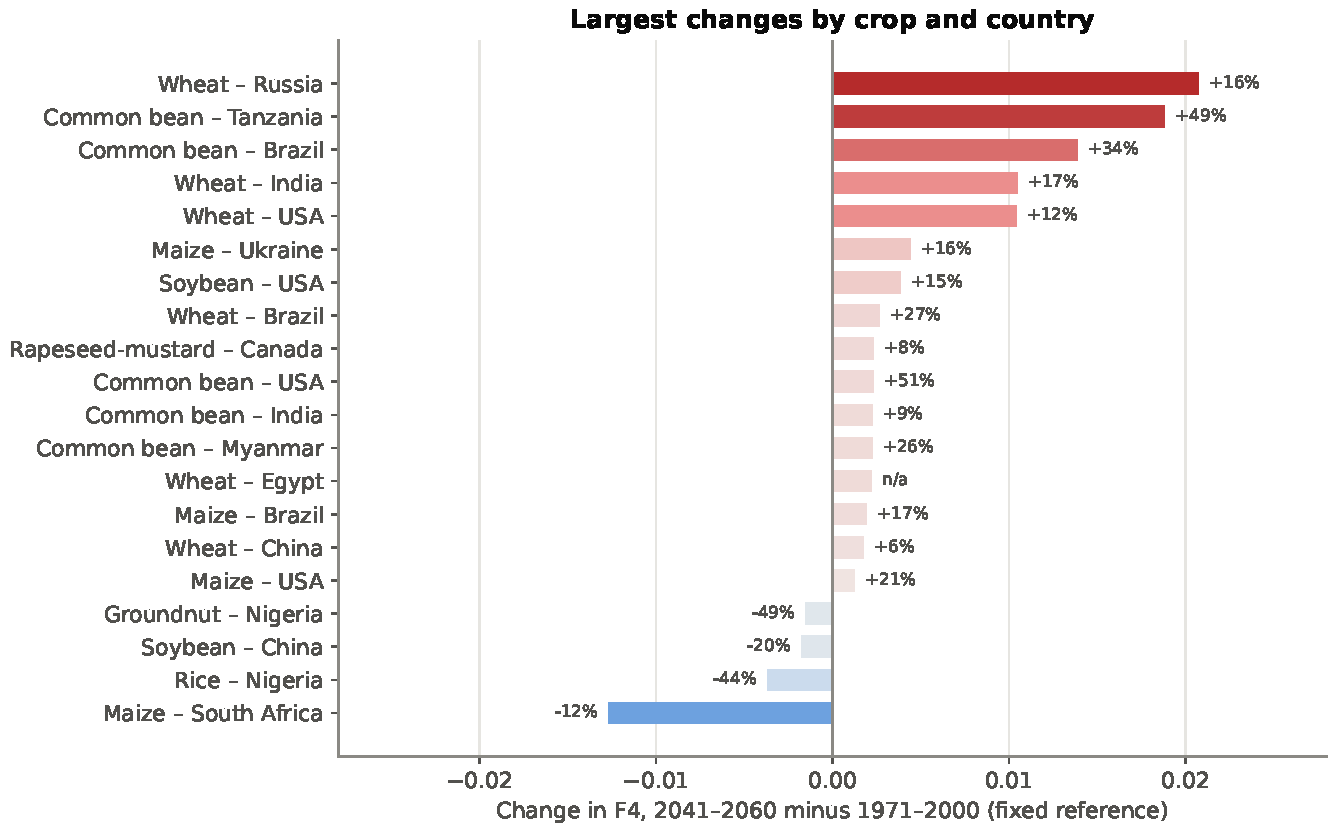
\includegraphics[width=0.85\linewidth]{G05_future_pairs.pdf}
\caption{Largest changes in pair scores, split into heat and water parts.}\label{fig:futurepairs}\end{figure}

\subsection{Does the result depend on the method?}
The climatology check applies the thresholds directly to the 20-year means instead of using change factors. It
gives the same sign of change in \climCheckSameSign\% of pairs, with Spearman $\rho$ = \climCheckRho\ between the
two sets of changes. The direction of change therefore does not hinge on the change-factor choice. It does depend
on the single climate model: the wetter South African maize season, for example, is a property of MRI-ESM2-0, and
other models disagree on regional rainfall.

\subsection{Interpretation}
A crop can stay nutritionally important while its climate stress rises, and a low score can still reflect the
monthly heat measure. The future index values are scores relative to today's maxima, not yield losses. The yield
and nutrient consequences are estimated separately in Section~\ref{sec:futurenut}.
